\chapter{Data Analysis}

\MyQuote{In physics, you don't have to go around making trouble for yourself - nature
does it for you.}{Frank Wilczek}

QCD jets are the most common hard objects observed at inelastic collisions 
collisions at hadron colliders, with their cross section exceeding any other
physics process by orders of magnitude.  Measurement of inclusive jet cross
section provides the test for both QCD predictions and the detector
performance up to the momentum transfers not reachable by any other physics
processes. 

In this Chapter, I will describe the details of the double differential
inclusive jet cross section analysis, which I have done in this thesis.
I will begin with the characteristics of the Monte Carlo data, I have used.
These data together with the event selection criteria and matching procedure,
which description will follow, fully specify the input for the unfolding
procedure. Two approaches to the unfolding, which I have implemented in this
thesis, will be described and compared with each other. 

At the end of this Chapter, I will compare the results of my data analysis, with
the next-to-leading order perturbative QCD prediction of my supervisor. 

\section{Data Characteristics}

As the input, I have used Monte Carlo generated events of proton-proton collisions at
the center-of-mass energy $\sqrt{s} = 13\TeV$ with \textsc{Pythia8}
\cite{Pythia8} event generator using CT10 Parton Distribution Functions
\cite{CT10PDF} and ATLAS underlying event tune AU2 \cite{AU2}. QCD calculations
are done only to the leading order in
\textsc{Pythia8}. The response of the ATLAS detector on these events was
simulated with \textsc{Geant4} \cite{Geant4} software toolkit.

Particles were recombined into jets using anti-$k_t$ jet algorithm with parameter $R=0.4$.
There are particle jets reconstructed from the \textsc{Pythia8} output, which
further in this thesis are denoted truth jets, and next to them, there are the
reco jets reconstructed from the output of \textsc{Geant4} detector
simulation from the ATLAS detector topological cell clusters. 

I have calibrated reco jets using the \textsc{ApplyJetCalibration}
\cite{ApplyJetCalibration} library v3.28 with configuration 
\texttt{JES\_Prerecommendation2015\_Feb2015.config} and
calibration sequence \texttt{JetArea\_Residual\_EtaJES}. In next, reco jets
denote the reco calibrated jets.

Events were generated in slices according to the leading truth jet $\pt$. These
samples differ in event weight which is for the whole event calculated as 

\begin{equation}
  \text{weight} = \frac{\text{(XS)} \cdot \text{(FE)} \cdot w_0}{\text{(\# events)}},
\end{equation}
with XS beeing cross-section, FE filter efficiency and $w_0$ additional weight
factor stored in \texttt{EventInfoAux} container. Concrete values for datasets used in
this theses are given in Table~\ref{tab:JZXW}.  

\begin{table}
  \centering
  \begin{tabular}{|c|rcr|c|c|c|}
    \hline 
     JZXW & \multicolumn{3}{|c|}{$\pt$ range (GeV)} & Cross-section (fb) & Filter Efficiency & \# events  \\ 
    \hline
    \hline
		 JZ0W &     0 & - &    20 & 7.8420e+13 & 9.7193e-01 & 3498000 \\ 
    \hline
		 JZ1W &    20 & - &    80 & 7.8420e+13 & 2.7903e-04 & 2998000 \\
    \hline
		 JZ2W &    80 & - &   200 & 5.7312e+10 & 5.2261e-03 & 500000  \\
    \hline
		 JZ3W &   200 & - &   500 & 1.4478e+09 & 1.8068e-03 & 499500  \\
    \hline
		 JZ4W &   500 & - &  1000 & 2.3093e+07 & 1.3276e-03 & 477000  \\
    \hline
		 JZ5W &  1000 & - &  1500 & 2.3793e+05 & 5.0449e-03 & 499000  \\
    \hline
		 JZ6W &  1500 & - &  2000 & 5.4279e+03 & 1.3886e-02 & 493500  \\
    \hline
		 JZ7W &  2000 & + &       & 9.4172e+02 & 6.7141e-02 & 497000  \\
    \hline 
  \end{tabular}
  \caption{The cross-sections (XS), filter efficiency (FE) and number of events
  for the JZXW samples which differ in the leading truth jet $\pt$ range.}
  \label{tab:JZXW}
\end{table}

In the analysis, I am using jets with transverse momentum $\pt>15\GeV$ and
rapidity $|y|<4$. Analysis is done in double binning in $\pt$ and $|y|$, with
the edges being the same as in the analysis from 2011/2012 \cite{Analysis2012},
which has chosen the binning in $\pt$ to uncertainty in each bin was smaller
than the differences in values in neighboring bins.

\begin{align}
  \pt = \, &15-20-25-35-45-55-70-85-100-116-134-152- \nonumber \\
        &172-194-216-240-264-290-318-346-376-408- \nonumber \\
        &442-478-516-556-598-642-688-736-786-838- \nonumber \\
        &894-952-1012-1076-1162-1310-1530-1992-2300- \nonumber \\
        &2800-3400-4100-5000-6000-7200 \GeV \nonumber \\
  |y| = \, &0.0-0.5-1.0-1.5-2.0-2.5-3.0-3.5-4.0
  \label{eq:Binning}
\end{align}

\section{Event Selection}

In this section the jet selection criteria and matching of truth with reco
jets are described. The former is needed to cut those jets (or those events)
off, which were misinterpreted by the detector, by the later the inputs for the
unfolding procedure are obtained. Description of the unfolding procedure will
follow in the next section. More details including graphical display and
numerical results for procedures described in this section are given in Appendix
\ref{App:CutAndMatchingResults}.

\subsection{Jet Cuts}
\label{SubSec:JetCuts}

\begin{itemize}
  \item \textbf{$\mathbf{\pt}$ Cut}

    Reco and truth jets with $\pt > 15 \GeV$ were kept.

  \item \textbf{$\mathbf{y}$ Cut}
    
    Reco and truth jets with $|y| < 4$ were kept.

  \item \textbf{Zero jet (0-jet) Cut}

    Only those events which has at least one reco or one truth jet are
    considered.
    
  \item \textbf{Leading Ration (LR) Cut}

    In this cut the reco and truth jets with the highest $\pt$ were used. If
    there was only one reco jet left, the ratio $LR = \pt^{reco,leading} /
    \pt^{truth,leading}$ was calculated. If there were two reco jets, instead
    of $\pt^{reco,leading}$ the average $\pt$ of two leading reco jets was
    calculated. If $0.6 < LR < 1.4$ the event are considered.

\end{itemize}

Numbers of reco and truth jets removed in each step are shown in Table
\ref{tab:CutAndMatchingEfficiency}, where also the cut efficiencies for individual
JZXW samples are shown. The impact of each cut on jet $\pt$ spectrum of reco
and truth jets is displayed in Figure \ref{fig:Cutting}. 

It can be seen that the most important cut is the 0-jet cut which removes
approximately $80\,\%$ of reco jets in JZ0W sample whereas the truth jets
remain intact. According to Table \ref{tab:JZXW} for event from the JZ0W sample
the leading truth jet $\pt < 20 \GeV$ which has no longer to hold for reco
jets which were in some cases reconstructed with $\pt \sim 100 \GeV$. Because of
Monte Carlo event weight of events from JZ0W sample is dominant over event
weights of other JZXW samples by several orders, the misreconstructed reco
jets from JZ0W sample were negatively influencing the observed $\pt$ spectrum of
reco jets as can be seen from top of the Figure \ref{fig:Cutting}.

\subsection{Jet Matching}
\label{SubSec:JetMatching}

To find, how the truth jets are reconstructed by the detector, the jet matching
has to be done, i.e. for each truth jet it is needed to find corresponding reco
jet. Jet matching used in this thesis is based on minimal angular distance
between matched and its description follows in this section.

For each pair $(i,j)$ of reco and truth jet, the quantity $dR_{ij} =
\sqrt{d\phi_{ij}^2 + dy_{ij}^2}$ was calculated with $d\phi_{ij}$ being angle
between $\phi_i^{reco}$ and $\phi_j^{truth}$ and $dy_{ij} = y_i^{reco} -
y_j^{truth}$.  The minimum was found between all of $dR_{ij}$'s. If this was
smaller than the defined cutoff $\min(dR_{ij}) = dR_{pq} < dR^{cutoff} = 0.2$,
the jets $(p,q)$ were matched and further not assumed in matching procedure.
This continued until condition $\min(dR_{ij}) < dR^{cutoff}$ was not satisfied
or all of the reco or truth jets were matched.

Numbers of reco and truth jets, both matched and unmatched are shown in Table
\ref{tab:CutAndMatchingEfficiency} where also the matching efficiencies for
individual JZXW samples are shown. Figure~\ref{fig:Matching} shows the $\pt$
spectra of truth and reco jets after event selection, which are composed from
$\pt$ spectra of matched and unmatched jets, which are shown also. $\pt$ spectra
of truth and reco jets are for all rapidity bins assumed in this thesis shown in
Figure~\ref{fig:ptSpectraMasacreEverythingFuck}.

\begin{figure}[t]
  \centering
  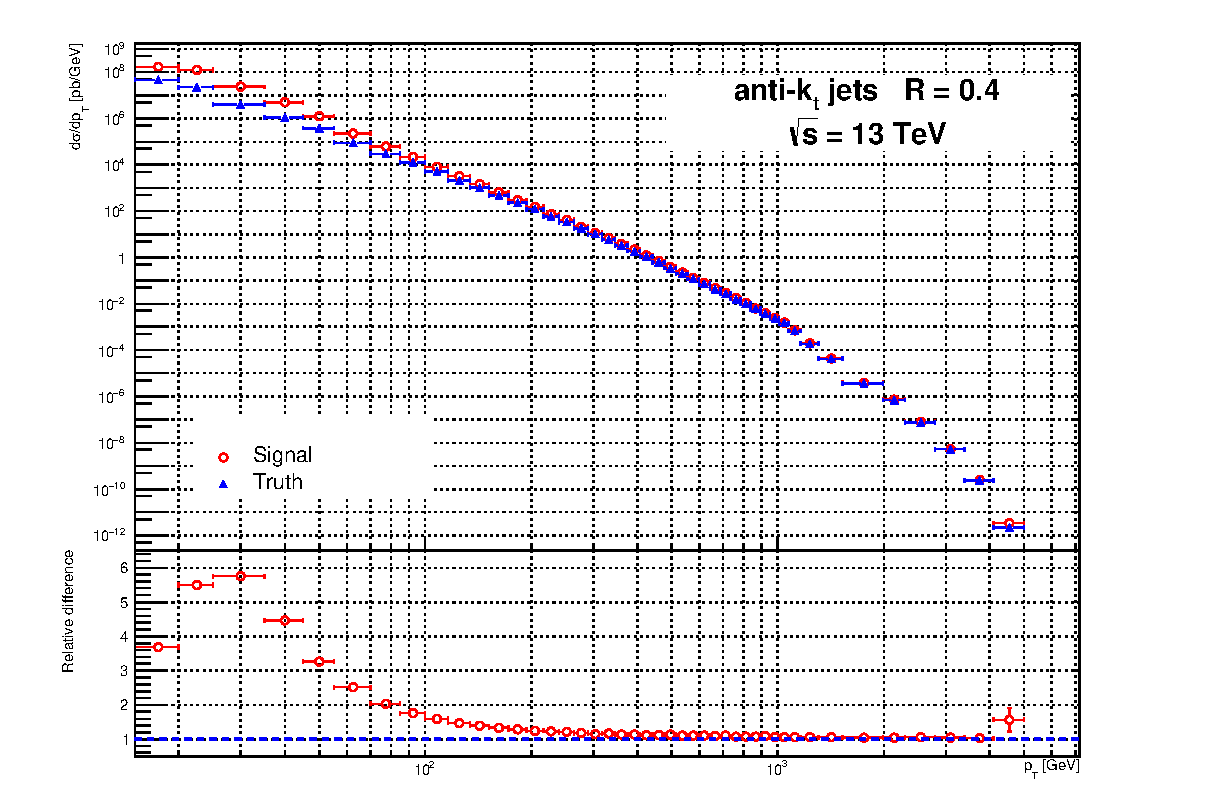
\includegraphics[width=\textwidth]{{Chapter3/SignalVSTruth}.eps}
  \caption{Comparison of $\pt$ spectra of reco and truth jets after event
    selection for selected $|y|<0.5$ rapidity bin. Each $\pt$ bin was divided by
    its width so $y$-axis has physical meaning of double differential cross
    section in $\pt$ and $y$.  Bottom graph contains the relative difference
    between reco and truth cross sections.} 
  \label{fig:SignalVSTruth}
\end{figure}

\section{Unfolding}
\label{Sec:Unfolding3}

After the four cuts from section~\ref{SubSec:JetCuts}, the sets of jets
denoted reco and truth jets were obtained. Matching procedure, described in
section~\ref{SubSec:JetMatching},
divided both reco and truth jets into two categories depending on successful
matching - there is correspondence 1 : 1 between matched reco and matched truth
jets. Reco jets, which were not matched, formed the unmatched reco jets, and
similarly a set of unmatched truth jets was created. All these 6 sets of jets
are needed by the unfolding procedure which description follows in this section.

Figure~\ref{fig:SignalVSTruth} shows the $\pt$ spectra of reco and truth jets.
It can be seen, that observed $\pt$ spectrum, represented by the reco jets,
differs from the $\pt$ spectrum theoretically expected which is represented by
the $\pt$ spectrum of truth jets. Unfolding should transform the observed $\pt$
spectrum to the spectrum theoretically expected. If this transformation would be
done on real data, it should ideally preserve additional structures, which are
presented in data, but not included by the theory.


The main ingredient for the unfolding procedure is the transfer matrix $A_{ij}$
which contains the number of reco jets in bin $i$ with a matched truth jet that
was generated in bin $j$ and describes thus the smearing effects of the
detector. In this thesis, the double binning \eqref{eq:Binning} is used which
complicates the situation because the matched reco jet can simply migrate of the
transfer matrix from Figure~\ref{fig:UnfoldingMatrixDetail}, when, for example,
its rapidity $|y|>0.5$ and when it was matched with truth jet with $|y|<0.5$ or
vice versa. Two ways of dealing with double binning are tested in this thesis.

\begin{enumerate}
  \item \textbf{Simple unfolding}
    
    In this case, only those reco and truth jets were used in the transfer
    matrix, which were matched within the same rapidity bin. Remaining matched
    jets were added to the unmatched jets. 8 transfer matrices $46 \times
    46$ are filled (one for each rapidity bin, $46$ = number of $\pt$ bins) and
    unfolding is done for each of these matrices separately. One of these
    matrices for $|y|<0.5$ rapidity bin is shown in
    Figure~\ref{fig:UnfoldingMatrixDetail}.

  \item \textbf{2D unfolding}

    In this case, the unfolding matrix was redefined to encapsulate the matching
    of jets between different rapidity bins. In this case only one transfer
    matrix $368 \times 368$ is created ($368 = 46 \times 8$) with unfolding being
    done only for this matrix shown at Figure~\ref{fig:UnfoldingMatrixAll}, from which
    the way how the transfer matrix was redefined from the simple unfolding
    should follow. 
\end{enumerate}

\begin{figure}[p]
  \centering
  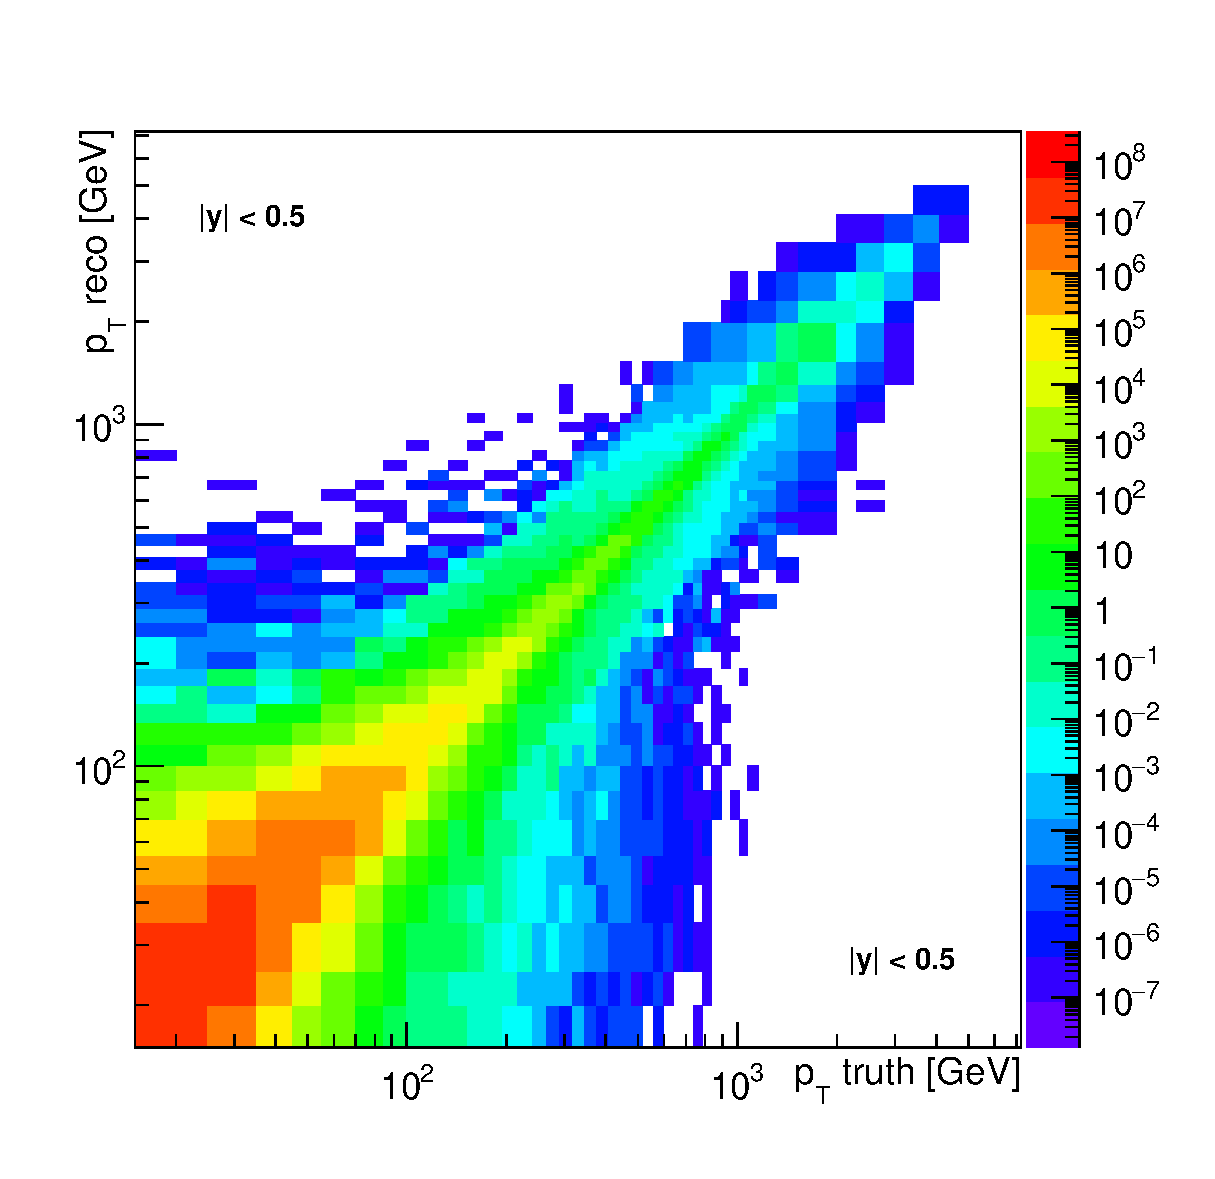
\includegraphics[width=\textwidth]{{Chapter3/Unfold_matrix_firstBin}.eps}
  \caption{Unfolding matrix for matched reco and truth jets with rapidity
  $|y|<0.5$ corresponding to one of eight matrices used in the simple unfolding.
  Each cell is proportional to the number of jets with truth $\pt$ in range
  determined by the $x$-axis which were reconstructed to the reco jets
  with $\pt$ determined by the $y$-axis. White space signalize no input.}
  \label{fig:UnfoldingMatrixDetail}
\end{figure}

\begin{figure}[p]
  \centering
  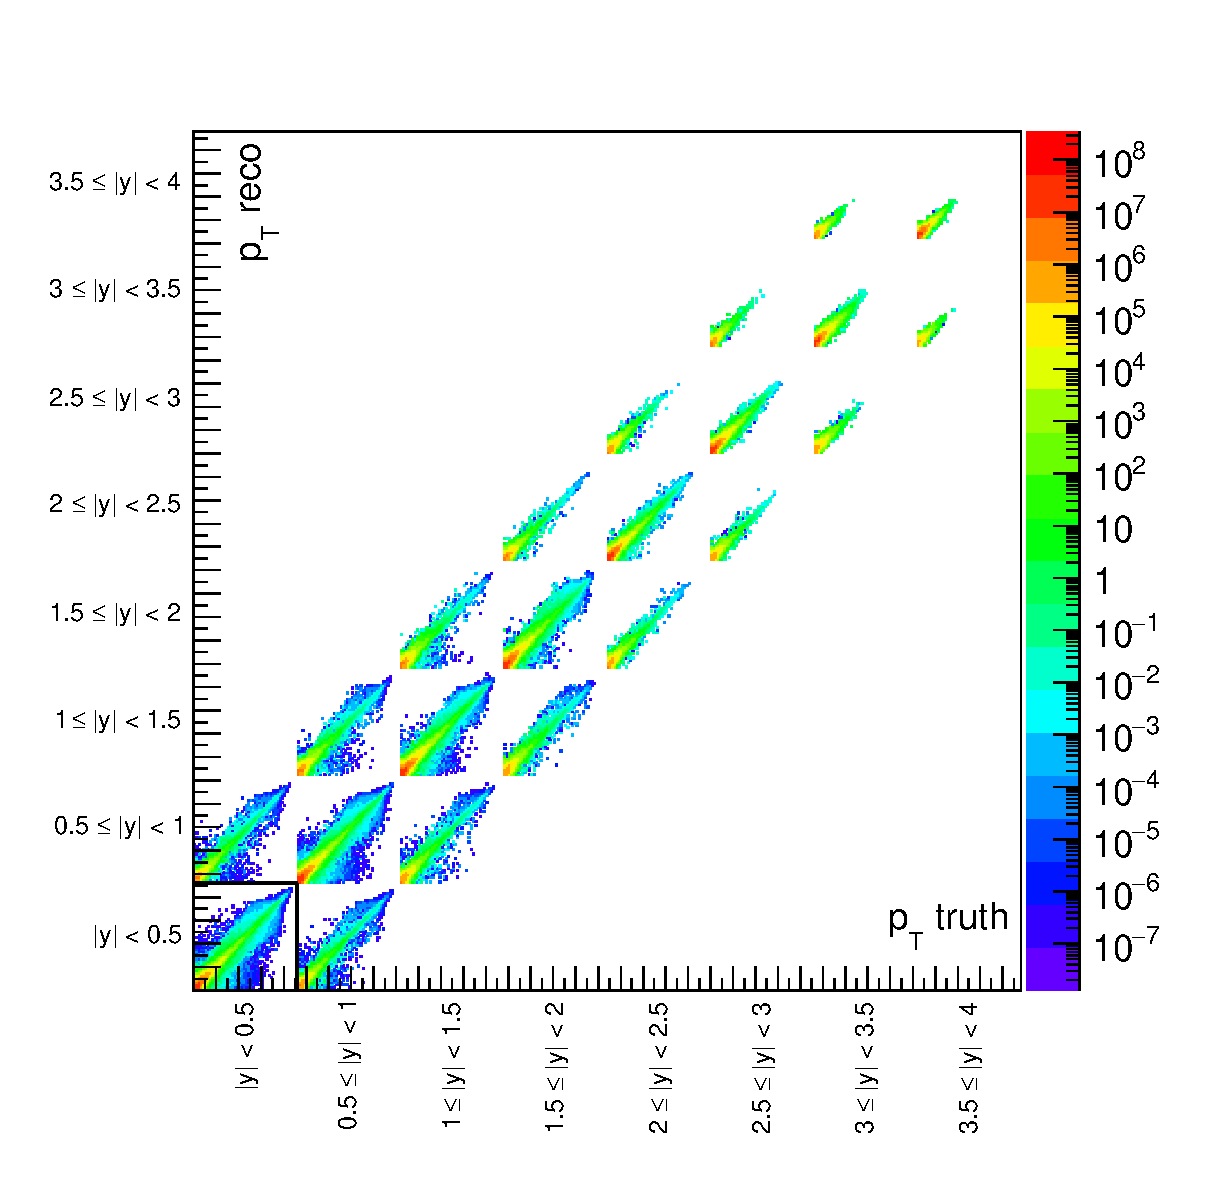
\includegraphics[width=\textwidth]{{Chapter3/Unfold_matrix_all}.eps}
  \caption{Unfolding matrix used in the 2D unfolding. Each cell is
    proportional to the number of jets with truth $\pt$ and rapidity $y$
    determined by the $x$-axis, which were reconstructed to the reco jets with
    $\pt$ and $y$ determined by the $y$-axis. Marked square in $|y|<0.5$ region
    is the matrix shown in Figure \ref{fig:UnfoldingMatrixDetail}. Projection of
    this matrix on the $x$ and $y$-axis corresponds to the $\pt$ spectrum of
    matched truth and reco jets for corresponding rapidity bin respectively.
    Projections on $y$ axis are shown in
    Appendix~\ref{sec:UnfoldingMatrixSlices}.} 
  \label{fig:UnfoldingMatrixAll}
\end{figure}

Transfer matrix from Figure~\ref{fig:UnfoldingMatrixAll} used by the 2D
unfolding contains at the diagonal 8 submatrices which are the unfolding
matrices used by the simple unfolding. Next to these diagonal submatrices
transfer matrix of 2D unfolding contains 14 additional submatrices beside
diagonal. These corresponds to the matched jets with migration in rapidity bins
and in case of simple unfolding, these jets are assumed to be unmatched.
Appendix~\ref{sec:UnfoldingMatrixSlices} shows some of the
    slices in the transfer matrix of 2D unfolding.

Dominant elements of each of the submatrices are on the main diagonal, which
corresponds to the fact, there is no significant bias in $\pt$ reconstruction.
The finite $\pt$ resolution causes the smearing of the diagonal and finite
rapidity resolution is the cause of the 14 minor submatrices.
Appendix~\ref{sec:UnfoldingMatrixSlices} shows the slices in transfer matrix of
2D unfolding which demonstrates the facts just stated.

Next to the transfer matrix, numbers of matched and unmatched reco and truth
jets are needed for each $(y,\pt)$ bin by unfolding procedure. These serve for
calculation of matching efficiency which is the key ingredient in the first and
the last step of unfolding procedure. Matching efficiencies for $|y|<0.5$
rapidity bin are for both simple and 2D unfolding shown in
Figure~\ref{fig:MatchingEfficiencyDemonstration} and for other rapidity bins,
the results are shown in Appendix~\ref{sec:MatchingEfficiency}

\begin{figure}[p]
  \centering
  \makebox[\textwidth][c]{
    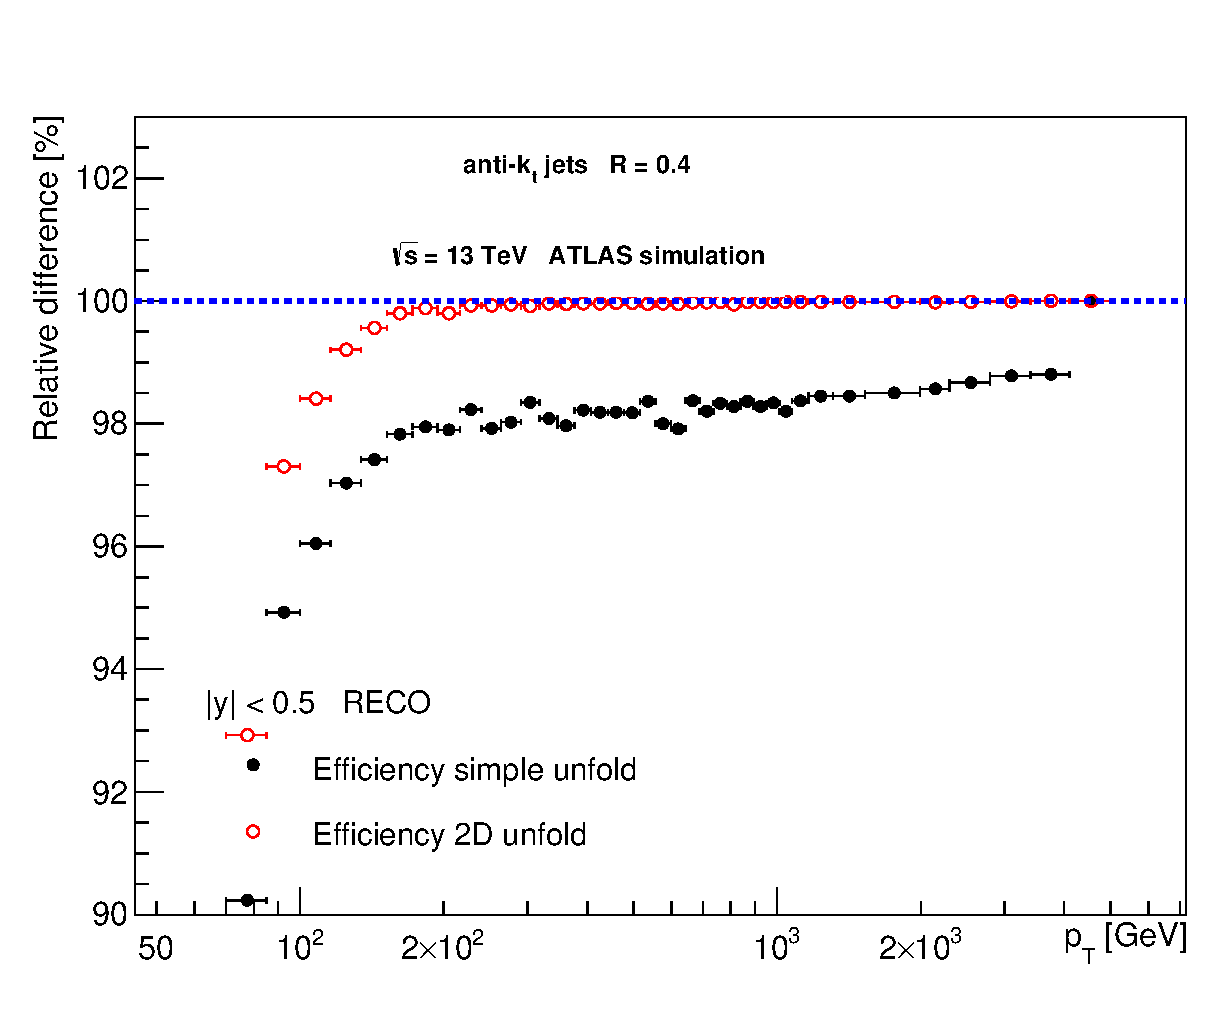
\includegraphics[width=0.6\textwidth]{{Chapter3/MatchEffSimpe2DSignal0Compare}.eps}
    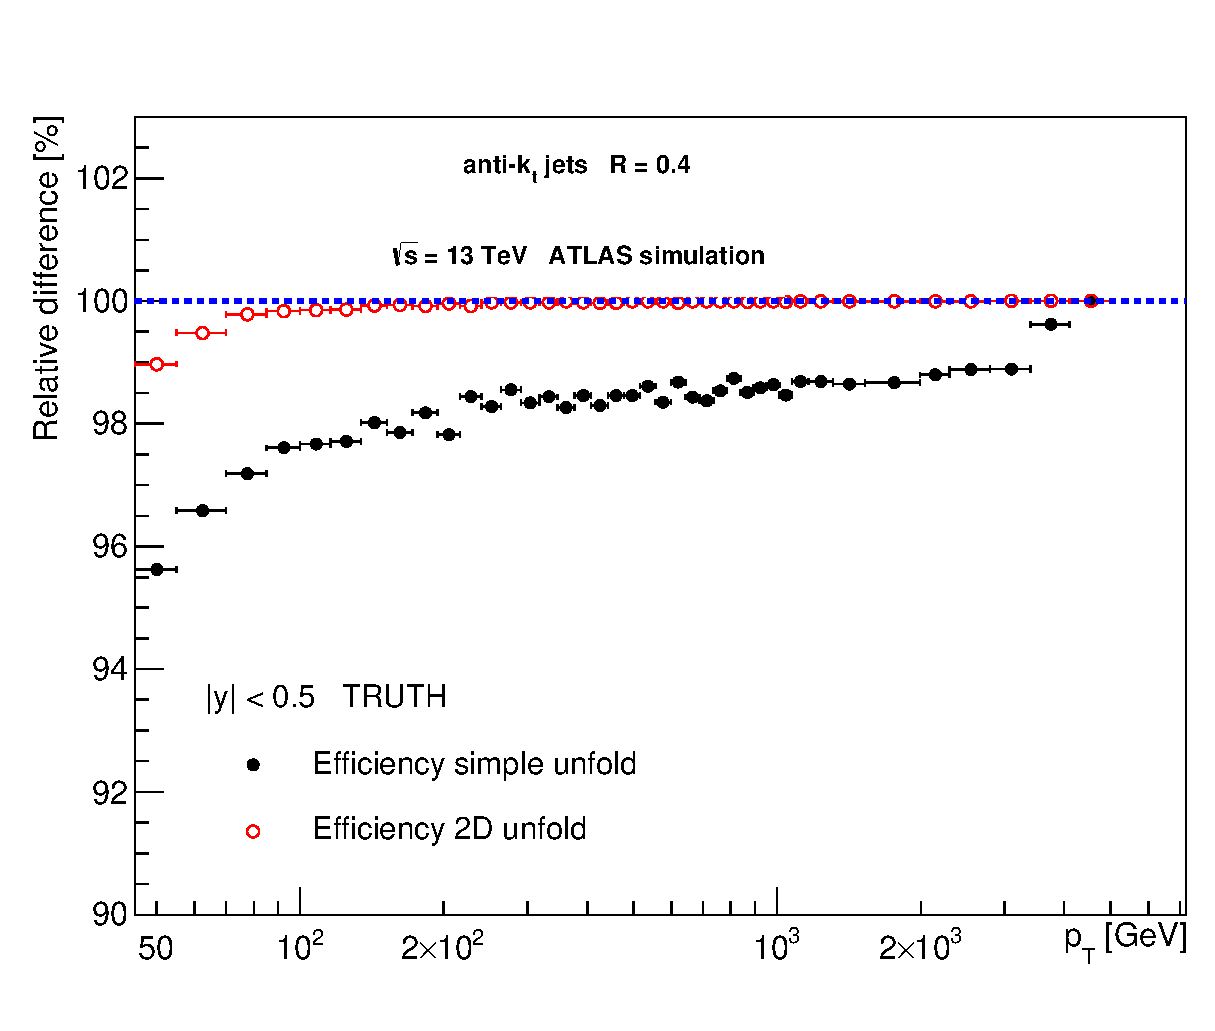
\includegraphics[width=0.6\textwidth]{{Chapter3/MatchEffSimpe2DTruth0Compare}.eps}
  }
  \caption{Comparison of matching efficiency of simple and 2D unfolding for $|y|
    < 0.5$ rapidity bin. Matching efficiency is compared for both reco jets
    (left) and truth jets (right). Matching efficiency for all rapidity bins is
    shown in Appendix \ref{sec:MatchingEfficiency}.}
  \label{fig:MatchingEfficiencyDemonstration}

  \vspace{1cm}
  
  \makebox[\textwidth][c]{
    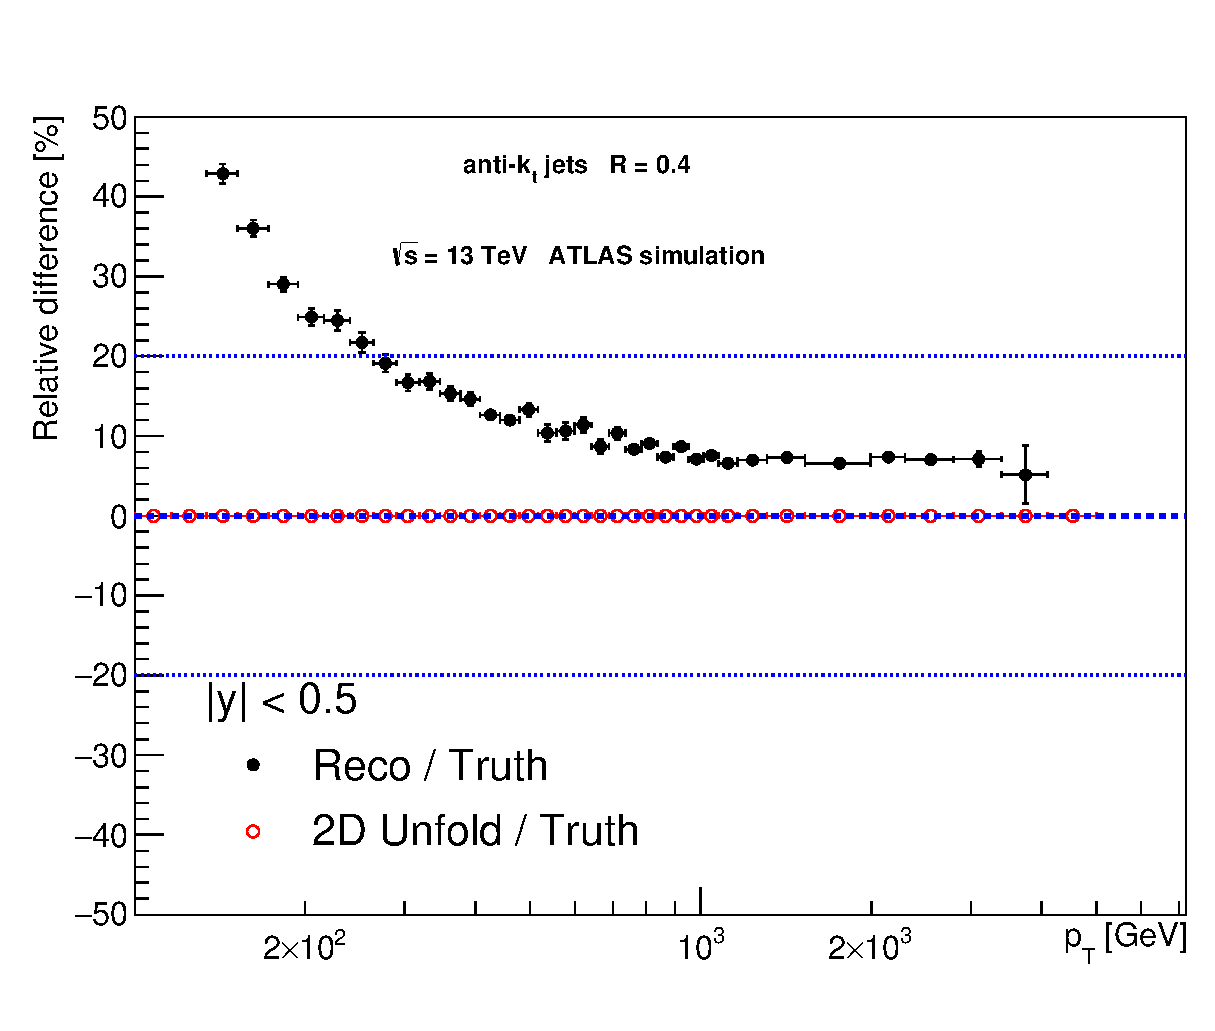
\includegraphics[width=0.6\textwidth]{{Chapter3/SignalUnfolded_VS_Truth0Compare}.eps}
    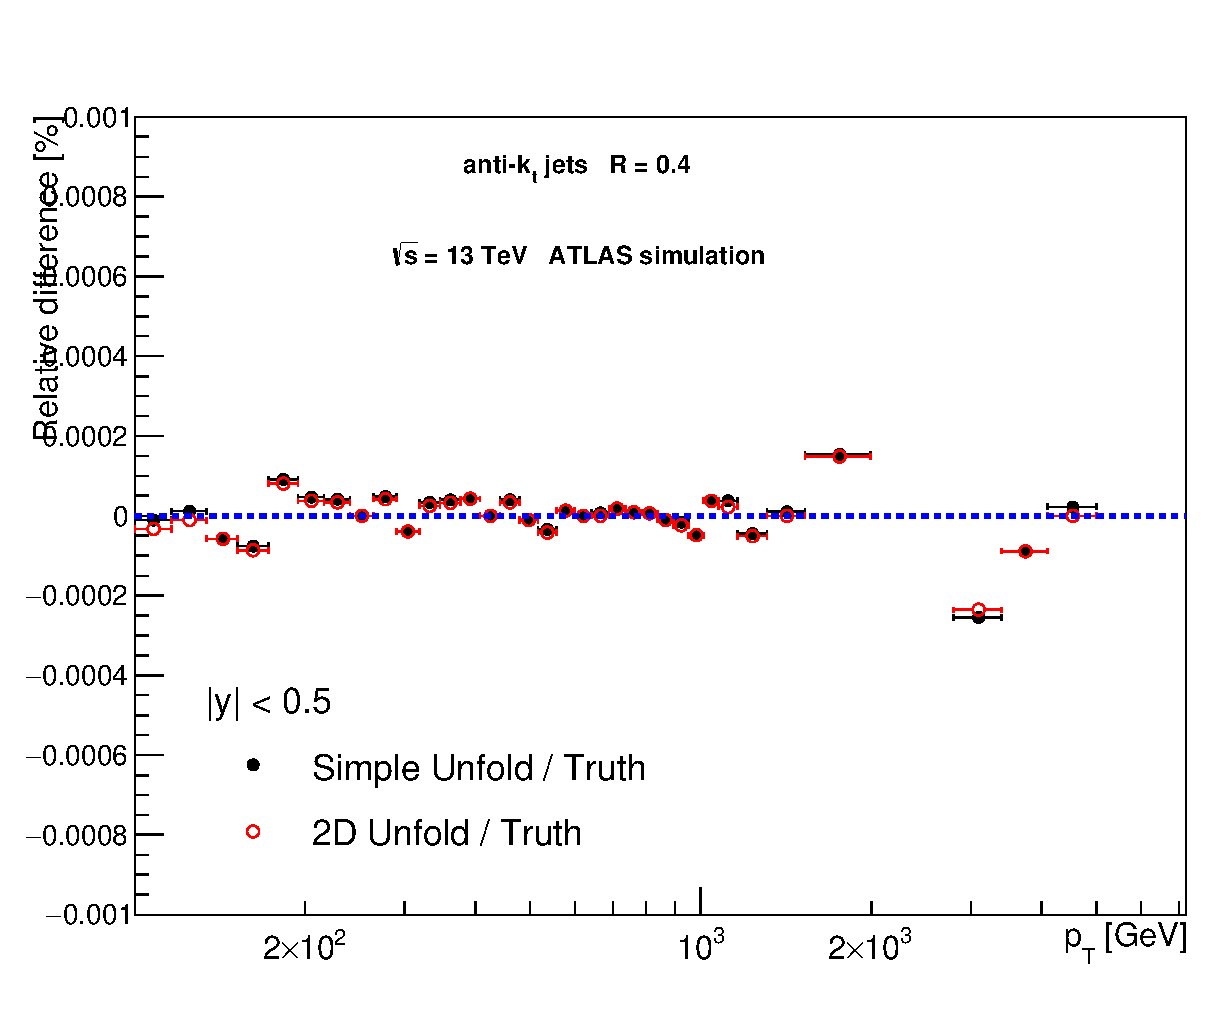
\includegraphics[width=0.6\textwidth]{{Chapter3/UnfoldedSimpleComplex_VS_Truth0Compare}.eps}
  }
  \caption{Comparison of $\pt$ spectra of reco jets and the unfolded
    $\pt$ spectra (2D unfolding) with the $\pt$ spectra of the truth jets
    (left). Comparison of unfolded spectra obtained by the 2D and simple
    unfolding with the $\pt$ spectra of the truth jets (right). Both graphs are
    for $|y|<0.5$ rapidity regions. Results for all rapidity bins are shown in
    Appendices \ref{sec:UnfoldingResults}, \ref{sec:SimpleAnd2DUnfolding}. }
  \label{fig:UnfoldingResultsDemonstration}
\end{figure}


Unfolding procedure can be divided into three main steps

\begin{enumerate}
  \item Input data are multiplied by the matching efficiency of reco jets.
  \item Transfer matrix is used to correct data spectrum for detector effects.
    For this purpose, the Iterative Dynamical Stabilized (IDS)
    \cite{IterativeDynamicallyStabilized} unfolding method was used which uses
    the series of iterations to improve unfolding results. In this thesis the
    iteration was done once.
  \item Spectrum obtained by the step 2 is divided by the matching efficiency of
    truth jets in order to correct resulting spectrum for the unmatched truth
    jets.
\end{enumerate}

Figure~\ref{fig:UnfoldingResultsDemonstration} shows the comparison of $\pt$
spectra of reco jets and unfolded spectrum (by 2D unfolding method) with the
$\pt$ spectrum of truth jets (left) and the comparison of simple and 2D unfolded
spectra with the spectrum of truth jets (right) for $|y|<0.5$ rapidity bin.
Results for all rapidity bins are shown in Appendix \ref{sec:UnfoldingResults}.

From figures it follows, the unfolding procedure corrects the
$\pt$ spectrum of reco jets to $\pt$ spectrum of truth jets up to the systematic
error $<10^{-3}\,\%$ and that the differences between results of simple and 2D
unfolding are even smaller.

\section{Comparison with NLO Prediction}
\label{sec:ComaprisonWithNLOPrediction}

In the previous sections, I have described the jet calibration and the unfolding
procedures. These serve to remove the detector imperfections and correct the
reco jet $\pt$ spectrum to the truth jet $\pt$ spectrum. For this purpose I
have used the \textsc{Pythia8} generated events, which uses
the leading-order QCD calculations to simulate initial $pp$ collision.
Nowadays the QCD predictions are tested up to next-to-leading order and for
LHC Run II, new calculations assuming next-to-next-to-leading order QCD
processes are preparing \cite{NNLO1,NNLO2}.

My supervisor has determined the theoretical prediction of $\pt$ spectra of
parton jets using \textsc{NLOJET++} program v4.1.2 \cite{NLOJetProgram}. This
program computes the QCD processes up to next-to-leading order with CT10
parton distribution functions \cite{CT10PDF, Annecy}. In this thesis I have used
his computations for center-of-mass energies $\sqrt{s}=8\TeV$ and
$\sqrt{s}=13\TeV$, first corresponding to the LHC Run I and second to LHC Run
II. In this section I compare the truth jet $\pt$ spectrum from \textsc{Pythia8}
with the theoretical prediction of parton jet $\pt$ spectrum from
next-to-leading order QCD predictions of my supervisor.

NLO predictions were compared for two different center-of-mass energies of $pp$
collisions - first corresponding to the LHC Run I ($\sqrt{s}=8\TeV$) and second
to Run II ($\sqrt{s} = 13\TeV$).  This comparison is shown for $|y|<0.5$
rapidity bin in Figure \ref{fig:ComparePredictionsDemonstation}, where also the
differential cross section is multiplied by the $\pt$ bin width and by
the integrated luminosity of Run I ($20\,\text{fb}^{-1}$) and expected
integrated luminosity of Run II ($100\,\text{fb}^{-1}$) to obtain expected number
of jets observed in each $\pt$ bin. Comparisons for other rapidity bins are
shown in Appendix \ref{sec:PredictionsForRunIAndII}.

\begin{figure}[t]
  \centering
  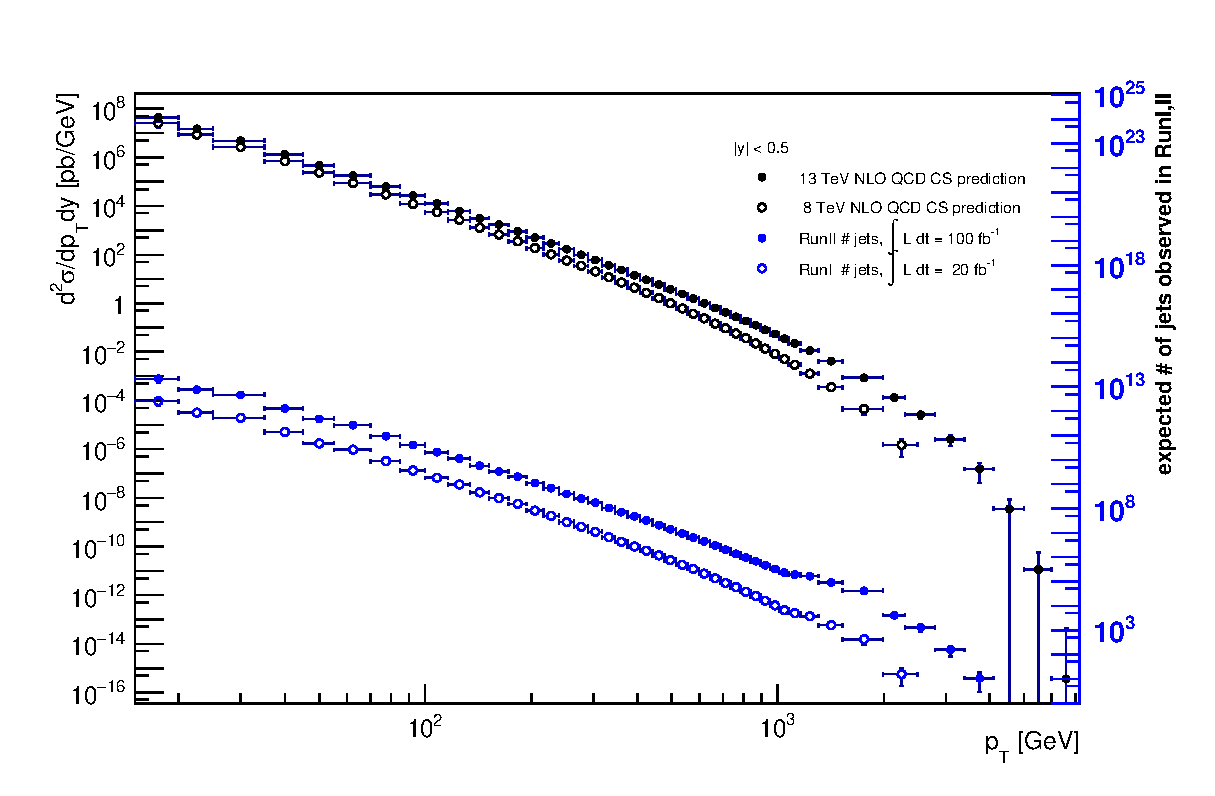
\includegraphics[width=\textwidth]{{Chapter3/PredictionCompare0}.eps} 
  \caption{Comparison of NLO QCD prediction of double differential inclusive jet
    cross section (black) for $pp$ collisions at $\sqrt{s}=13\TeV$ (filled circles)
    corresponding to the LHC Run II and $\sqrt{s}=8\TeV$ (empty circles)
    corresponding to the LHC Run I. The cross section is multiplied by
    integrated luminosities and $\pt$ bin width to obtain the expected number of jets
    observed in each $\pt$ bin (blue). Figure shows only $|y|<0.5$ rapidity bin,
    remaining rapidity bins are shown in Appendix \ref{sec:PredictionsForRunIAndII}.}
  \label{fig:ComparePredictionsDemonstation}
\end{figure}

It can be seen, that the increase in the center-of-mass energy is the most
significant for jets with high $\pt$. In the NLO QCD theoretical computations, several
uncertainties are taken into account. These include \cite{Analysis2012}

\begin{itemize}
  \item \textbf{Scale uncertainty}

    Coming from the choice of renormalization and factorization scales,
    including neglecting the higher order terms beyond NLO 

  \item \textbf{$\alpha_S$ uncertainty}

    Because $\alpha_S$ is experimentally determined with uncertainty.

  \item \textbf{PDF uncertainty}

    Prediction depends on the concrete choice of PDF.

  \item \textbf{Nonperturbative corrections uncertainty}

    Hadronization can split outgoing hard parton into a several jets. 

  \item \textbf{Electroweak corrections uncertainty}

    Next to the QCD processes, the electroweak processes has to be taken into
    account. These processes becomes more important, as the momentum transfer
    increases.  
\end{itemize}

\begin{figure}[t]
  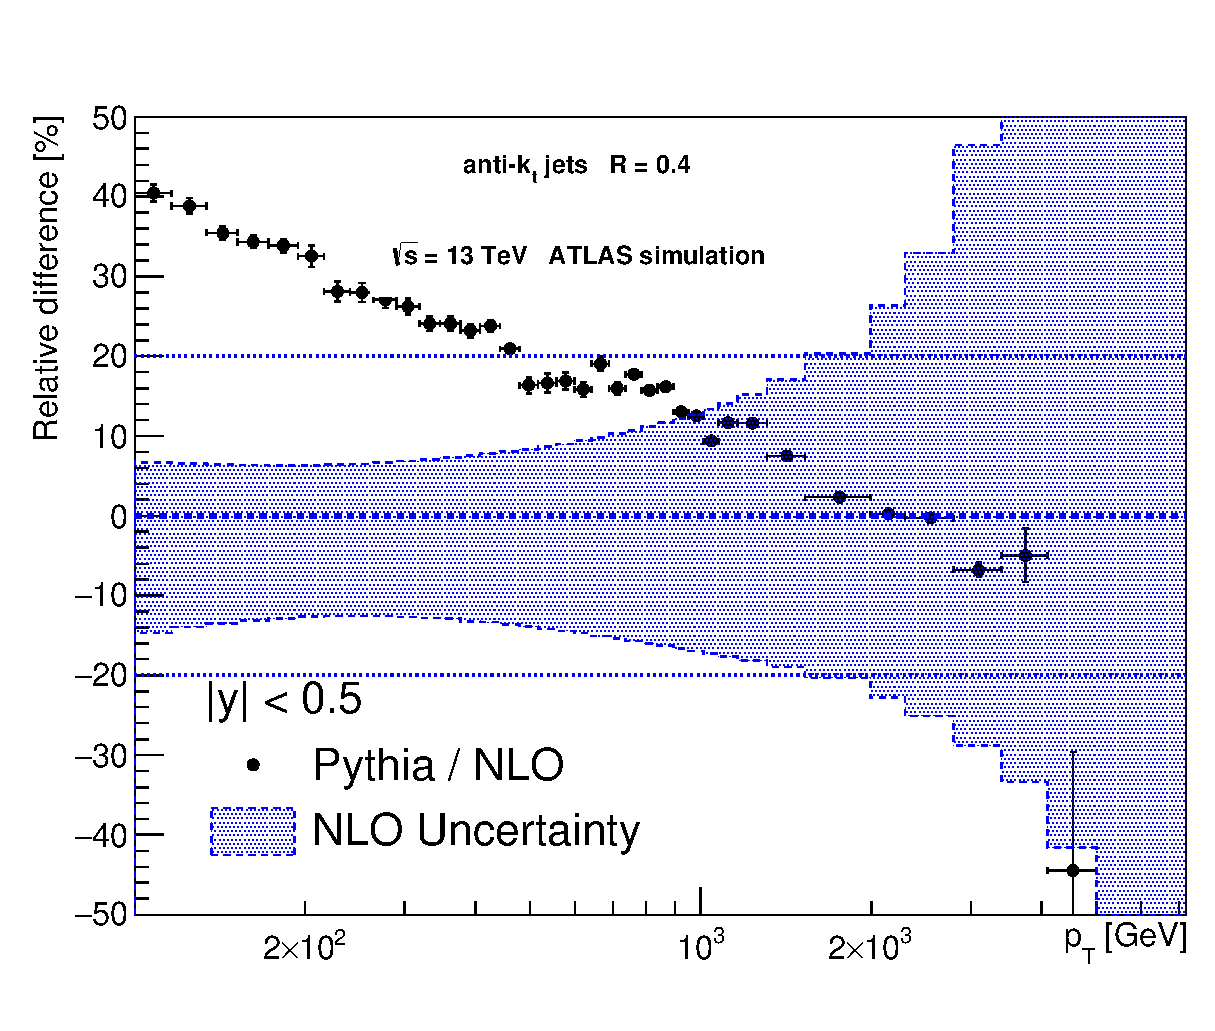
\includegraphics[width=\textwidth]{{Chapter3/Truth_VS_Prediction0Compare}.eps}
  \caption{Comparison of \textsc{Pythia8} prediction with NLO QCD prediction of
    inclusive jet double differential cross section for $|y|<0.5$ rapidity bin
    with uncertaintis of NLO QCD predictions symbolized by the blue area.
    Comparisons for other rapidity bins are shown in Appendix
    \ref{sec:PythiaAndNLO}.}
  \label{fig:TruthVSPredictionsDemonstation}
\end{figure}

In this analysis, only first three of these corrections are assumed. The
corrections were extracted from the files with NLO QCD predictions, where each
correction is represented by the set of equally likely histograms expressing the
deviation from the default prediction. Corrections are for $|y|<0.5$ rapidity bin
shown in Figure~\ref{fig:NLOSystematicsDemonstartion}, other rapidity bins
are shown in Appendix~\ref{sec:NLOUncertainties}.

\begin{figure}[p]
  \centering
  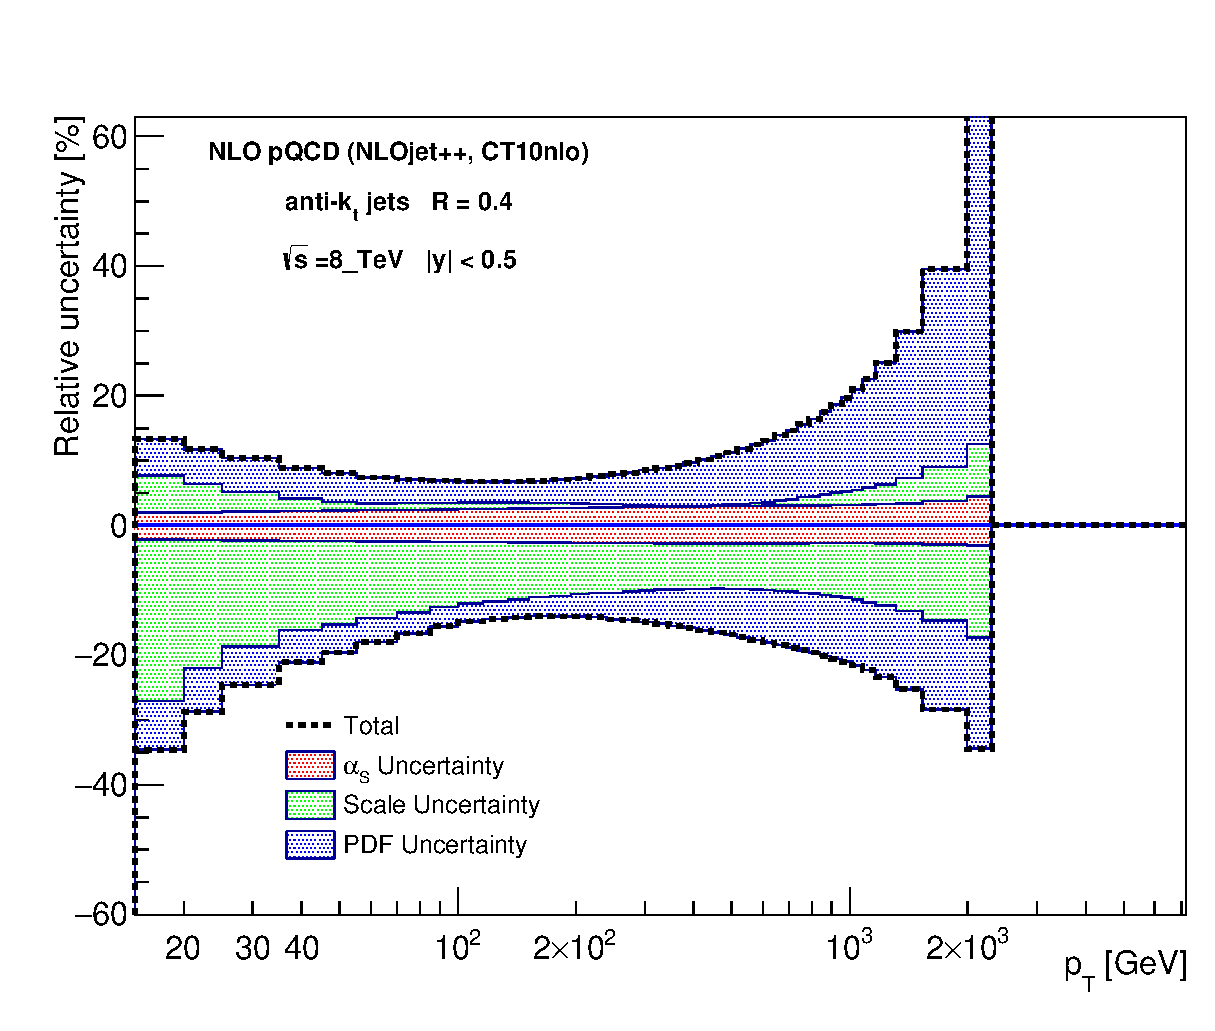
\includegraphics[width=\textwidth]{{Chapter3/NLO_Systematics8_TeV0}.eps}
  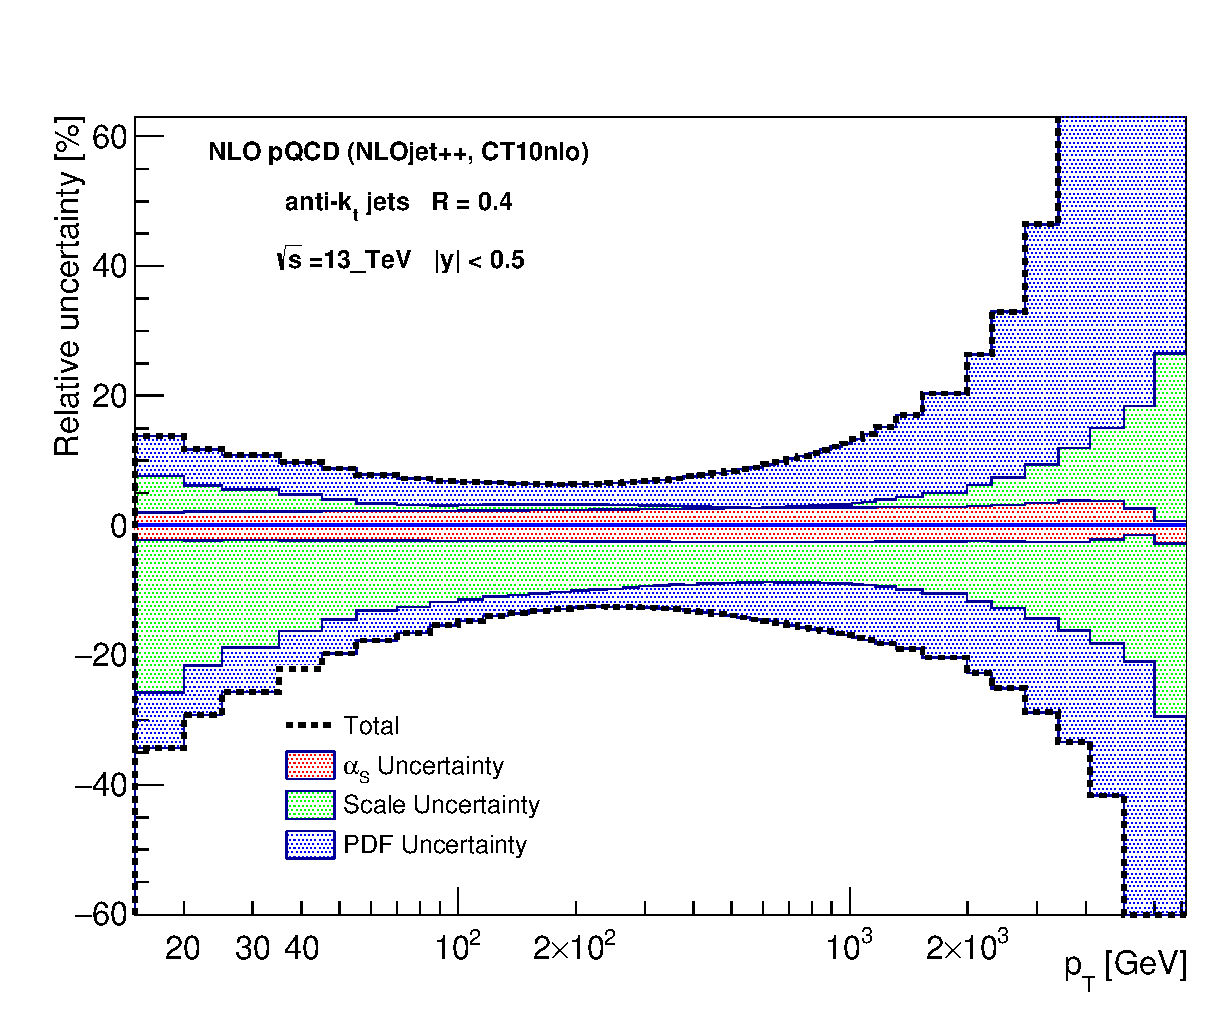
\includegraphics[width=\textwidth]{{Chapter3/NLO_Systematics13_TeV0}.eps}
  \caption{Theoretical uncertainties for NLO QCD predictions of inclusive jet
    differential cross section for $pp$ collisions at
    $\sqrt{s}=8\TeV$ (left) and $\sqrt{s}=13\TeV$ (right) for $|y|<0.5$ rapidity
    bin. Uncertainties for other rapidity bins are shown in Appendix
    \ref{sec:NLOUncertainties}.}
  \label{fig:NLOSystematicsDemonstartion}
\end{figure}

Comparison of $\pt$ spectra of truth jets with NLO QCD prediction is for $|y| <
0.5$ rapidity bin shown at Figure \ref{fig:TruthVSPredictionsDemonstation} for
other rapidity bins see Appendix \ref{sec:PythiaAndNLO}. It can be seen that the
truth $\pt$ spectrum is for low $\pt$ jet greater then the next-to-leading order QCD
prediction and that for a few $\pt$ bins with the highest $\pt$ the situation is
reversed. Physically, this is caused by the splitting of parton jet in the
process of hadronization into several truth jets.
